% !TeX root = ../main.tex
\section{Both Methods Work; One Keeps Working}
\label{sec:results}

\begin{table*}[t]
  \centering\small
  \begin{tabular}{@{}lrrrrrrrr@{}}
    \toprule
    & \multicolumn{3}{c}{\textbf{PTO}} & \multicolumn{3}{c}{\textbf{GRPO}}
    & \multicolumn{2}{c}{\textbf{PTO $-$ GRPO @10}}\\
    \cmidrule(lr){2-4}\cmidrule(lr){5-7}\cmidrule(lr){8-9}
    Metric & base & @10 & $\dz{}$ & base & @10 & $\dz{}$ & $\Delta$ & $\dz{}$\\
    \midrule
    \QQ{}~\emph{(reward)} & 3.00 & \textbf{4.26} & 1.43 & 3.07 & 3.75 & 0.72 & $+0.51^{***}$ & 0.73\\
    WAI-SR                & 2.85 & 3.50 & 0.97 & 2.89 & 3.44 & 0.84 & $+0.06^{\phantom{***}}$ & 0.12\\
    CSQ-8                 & 2.38 & 2.95 & 0.81 & 2.36 & 2.77 & 0.59 & $+0.17^{*}$   & 0.31\\
    MI-SAT                & 2.84 & 3.65 & 0.90 & 2.86 & 3.48 & 0.66 & $+0.17^{*}$   & 0.27\\
    MITI                  & 3.13 & 4.27 & 1.35 & 3.22 & 3.92 & 0.82 & $+0.35^{***}$ & 0.46\\
    PCT                   & 0.49 & 0.63 & 0.62 & 0.49 & 0.57 & 0.36 & $+0.06^{*}$   & 0.29\\
    \mici{}~$\downarrow$  & 0.21 & \textbf{0.49} & 0.78 & 0.21 & \textbf{0.84} & 1.72 & $-0.35^{***}$ & $-0.99$\\
    \bottomrule
  \end{tabular}
  \caption{Endpoint results at the matched tenth iteration, persona-paired over $n{=}96$.
  Left blocks: each arm's own base and its iteration-10 mean, with the paired $\dz{}$ of the
  gain over base (all Holm $p\!\approx\!0$). Right block: the paired PTO$-$GRPO difference
  at iteration~10 ($^{***}$ Holm $p<0.001$, $^{*}$ $p<0.05$; blank = n.s.). \mici{} is
  MI-\emph{inconsistency}, where lower is better, so its negative difference favours PTO.
  Primary grader (\primaryjudge{}).}
  \label{tab:endpoint}
\end{table*}

\begin{figure}[t]
  \centering
  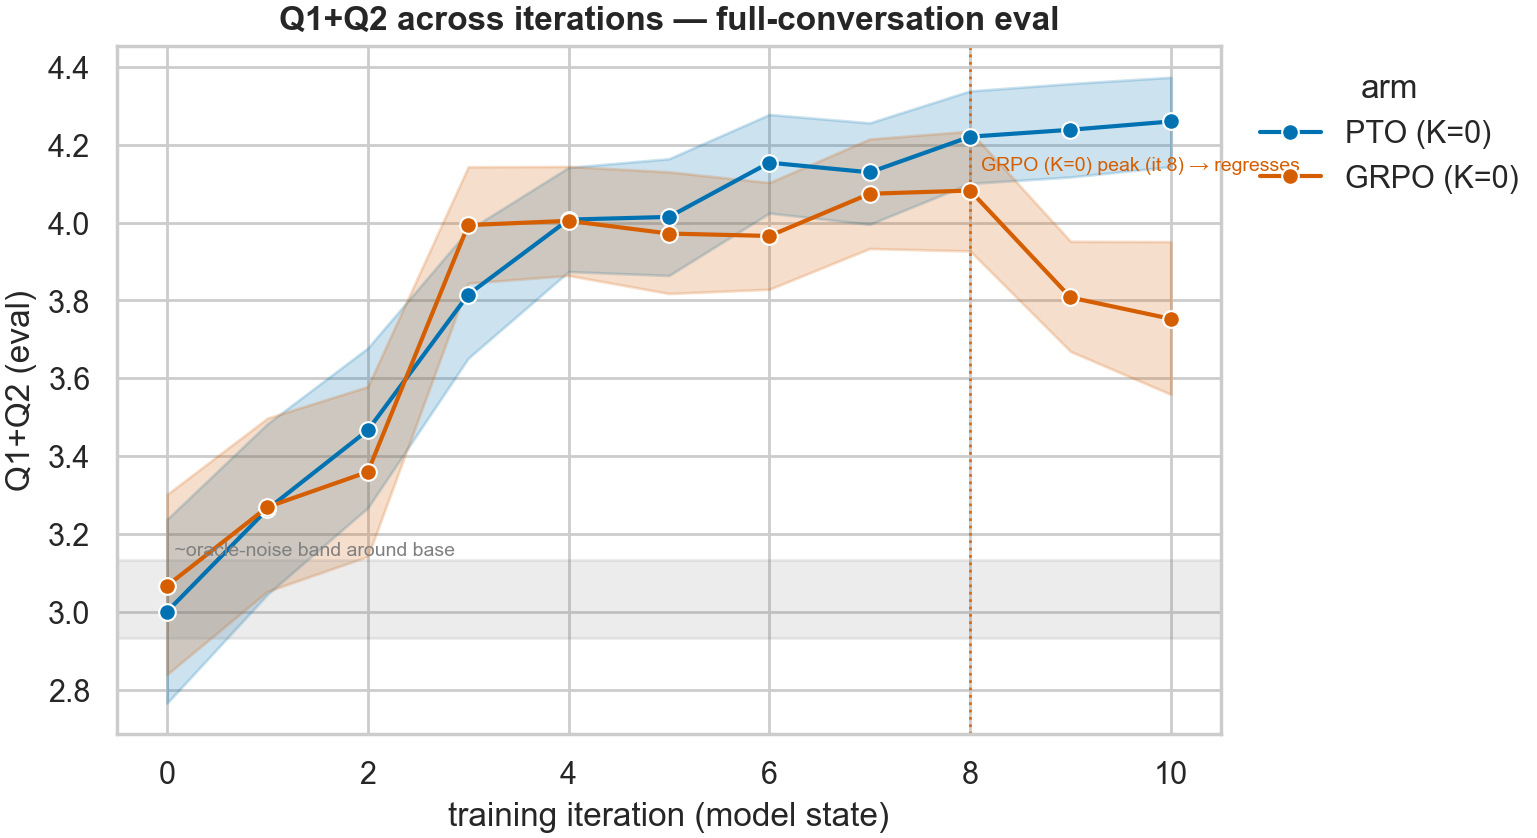
\includegraphics[width=\linewidth]{figures/trajectory_Q1Q2_gpt-4o-mini.png}
  \caption{\QQ{} (the training reward) across iterations, persona-paired means with 95\%
  CIs. PTO climbs monotonically to iteration~10; GRPO peaks at iteration~8 and regresses.
  Primary grader.}
  \label{fig:trajectory}
\end{figure}

\paragraph{Training works, and it works a lot.}
Both arms move the base 1B policy a long way. On the training reward, PTO goes
$3.00 \to 4.26$ ($\dz{}=1.43$) and GRPO $3.07 \to 4.08$ at its peak
($\dz{}=1.22$); every one of the five global rubrics is a large effect for PTO, with
Holm-corrected $p\!\approx\!0$ throughout (Table~\ref{tab:endpoint}). Degeneration is
eliminated: the base policy loops a verbatim therapist turn in $48$--$49\%$ of
conversations, and both arms drive that to $0$ by iteration~10. Sessions also lengthen
substantially per turn --- mean therapist turn length rises from ${\sim}270$--$300$ to
$686$ (PTO) and $896$ (GRPO) characters. Taken alone, this is a success story.

\paragraph{PTO leads at the matched endpoint, because GRPO regresses.}
At iteration~10 the paired difference is $+0.51$ \QQ{} in PTO's favour
($\dz{}=0.73$, Holm $p<0.001$), with MITI, MI-SAT, CSQ-8, PCT and \mici{} also favouring
PTO and only WAI-SR indistinguishable. The reason is visible in
Figure~\ref{fig:trajectory}: the two arms track each other for the first eight iterations
--- at iteration~8 the gap is only $+0.14$ --- and then diverge, because GRPO peaks at
iteration~8 ($4.08$) and falls to $3.75$ while PTO continues to $4.26$. Fitting a line
through each arm's trajectory gives $0.120$ \QQ{}/iteration for PTO against $0.072$ for
GRPO, with PTO's peak at its final iteration and GRPO's four iterations earlier.

We also report the \emph{steelman} comparison, since an experimenter with a validation set
would have stopped GRPO at its peak: PTO@10 still beats GRPO@8 by $+0.18$ \QQ{}
($\dz{}=0.30$, Holm $p=0.010$), along with CSQ-8, MI-SAT, WAI-SR and PCT; MITI and \mici{}
are indistinguishable at that pairing. So the ranking does not depend on GRPO's late
collapse --- but the \emph{size} of the ranking does, and honest reporting of an iterative
method should give both.

\paragraph{An iteration-9 dip, and what it is not.}
GRPO drops sharply at iteration~9 across nearly every metric simultaneously and partially
recovers at~10. We report it rather than smoothing it: it is a single-iteration event on
top of an already-monotonic decline from the iteration-8 peak, and \S\ref{sec:mechanism}
finds the same iteration flagged from a completely independent source (the training
signal), which argues it is a property of that update rather than a scoring artifact.

\paragraph{The rubrics are not eight independent measurements.}
Before reading Table~\ref{tab:endpoint} as ``PTO improved seven things,'' note that the
five global rubrics are an empirical redundancy cluster, not five constructs: they
co-load on a single principal component. With only those five, PC1 explains
${\approx}91\%$ of the variance. Adding the outside-the-reward metrics drops PC1 to
$55.0\%$ (GRPO) / $55.7\%$ (PTO) --- but the second factor is defined by \mici{} and the
MITI technique ratios, \emph{not} by patient change-talk, which correlates
$\rho \approx 0.79$--$0.94$ with the global cluster and therefore does not isolate MI
technique. In other words, ``all the rubrics went up together'' is close to one
measurement going up, which is precisely why the next section matters.
